\documentclass{beamer}
\usetheme{Dresden}

\usepackage{fontspec}
\usepackage{kpfonts}
\usepackage{graphicx}
\usepackage{pgfplots}
\usepackage{pgfplotstable}
\usepackage{tikz}
\usetikzlibrary{arrows,automata,mindmap,shapes,positioning,patterns,snakes,calc}

\pgfplotsset{every x tick label/.append style={font=\small, yshift=0.2ex}}
\pgfplotsset{every y tick label/.append style={font=\small, xshift=0.2ex}}


\usepackage{amsmath,amsthm,bm}
\usepackage{array}
\usepackage{color}
\usepackage{hyperref}

%\usepackage{algorithm}
%\usepackage{algpseudocode}
\usepackage{algorithm2e}


\hypersetup{
    colorlinks=true,
    linkcolor=blue,
    filecolor=blue,      
    urlcolor=blue,
}

\setbeamertemplate{caption}{\raggedright\insertcaption\par}
\usefonttheme[onlymath]{serif}
\usepackage{ragged2e}
\addtobeamertemplate{block begin}{}{\justifying}

\DeclareMathOperator*{\argmax}{\mathrm{\arg\max}}
\DeclareMathOperator*{\argmin}{\mathrm{\arg\min}}
\DeclareMathOperator*{\arginf}{\mathrm{\arg\inf}}
\DeclareMathOperator*{\argsup}{\mathrm{\arg\sup}}
\DeclareMathOperator{\sgn}{\mathrm{sgn}}
\DeclareMathOperator{\ind}{\mathrm{I}}
\DeclareMathOperator{\complex}{\mathrm{O}}
\DeclareMathOperator{\diag}{\mathrm{diag}}
\DeclareMathOperator{\prob}{\mathrm{Pr}}
\DeclareMathOperator{\var}{\mathrm{var}}
\DeclareMathOperator{\corr}{\mathrm{corr}}
\DeclareMathOperator{\cov}{\mathrm{cov}}
\DeclareMathOperator{\rand}{\mathrm{rand}}
\DeclareMathOperator{\vect}{\textit{vec}}
\DeclareMathOperator{\rank}{\textit{rank}}
\DeclareMathOperator{\tr}{\textit{tr}}


\title[]{Credit Allocation Problems}
\author[Chunheng Jiang, Ph.D in Computer Science]{Chunheng Jiang}
\date{}


\begin{document}

\begin{frame}
\titlepage
\end{frame}

\begin{frame}{Credit Allocation}
\begin{block}{}
Credit allocation is to solve the problem that how to allocate credits to the coauthors of a joint work.
It's a.k.a credit assignment.

\begin{itemize}
\item Collaboration among researchers is a vital component in academia.
\item No general guideline to place authors: contribution, seniority or alphabetical ordering.
\item Number of coauthors is increasing.
\end{itemize}

There are several common factors that affect the allocation, including \textit{the order of the coauthors}, \textit{the number of coauthors}~\cite{xu2016author} and \textit{the reputation in the community}~\cite{shen2014collective,bao2017dynamic}.
\end{block}
\end{frame}

\begin{frame}{Existing Methods}
\begin{block}{}
Shen and Barab{\'a}si~\cite{shen2014collective} developed a collective credit allocation procedure. It estimates the credits to the coauthors based on the votes from the whole community rather than the coauthors themselves.
\vskip 1em
Xu et. al.~\cite{xu2016author} investigated $15$ authors credit-assignment schemas. These schemas rely on the order of the coauthors and the total number of coauthors in the publications. These approaches present obvious similarity and strong correlation.
\vskip 1em
Based on~\cite{shen2014collective}, Bao and Zhai~\cite{bao2017dynamic} proposed to incorporate a reinforcement mechanism and a power-law temporal relaxation function.
\end{block}
\end{frame}

\begin{frame}{Shen's Method}
\begin{block}{}
\begin{itemize}
\item Target Paper: $p_0$
\item Authors: $\mathcal A=\{a_1,a_2,\ldots,a_m\}$
\item Papers Citing: $\mathcal D=\{d_1,d_2,\ldots,d_\ell\}$
\item Papers Co-cited: $\mathcal P=\{\textcolor{red}{p_0},p_1,p_2,\ldots,p_n\}$
\end{itemize}

The credit shares of a coauthor is determined by whether she continues working with other coauthors on the topic of $p_0$. Here, the set $\mathcal D$ plays as a committee from the same community, and the citations are their votes. A bipartite network can be constructed. 
\end{block}
\end{frame}

\begin{frame}{Shen's Method}
\begin{block}{}
The credit share of $a_i$ in $p_0$ is computed with the formula: 
\[c_i = \sum_{j=1}^n A_{ij}s_j,\]
where $A_{ij}$ is the credit $a_i$ earns from the cocited paper $p_j$, and each coauthor gets the same amount of shares from $p_j$. The relevance level (or cocitation strength) $s_j$ of $p_j$ to $p_0$ is defined as the number of documents in $\mathcal D$ referring both $p_0$ and $p_j$.
\end{block}
\end{frame}

\begin{frame}{Shen's Method}
\begin{figure}[ht]
\centering
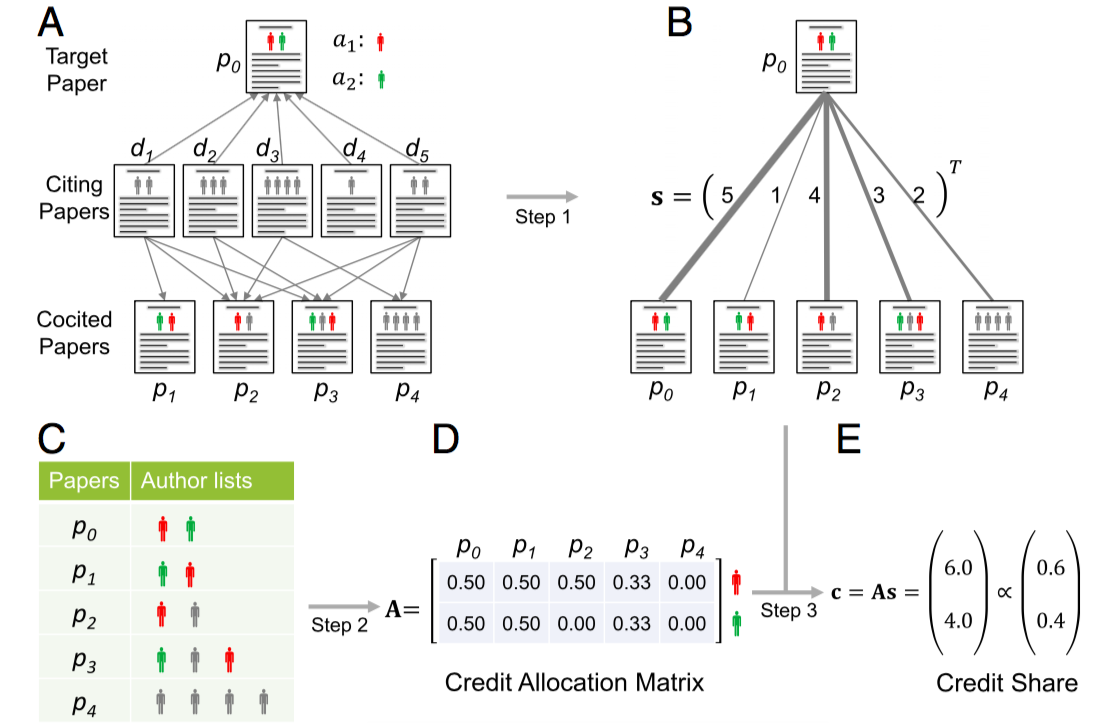
\includegraphics[scale=0.25]{figures/credalloc_algo}
\end{figure}
\end{frame}

\begin{frame}{Priors}
There are various author-list based prior rules to construct the credit allocation matrix $A$: 
\begin{figure}[ht]
\centering
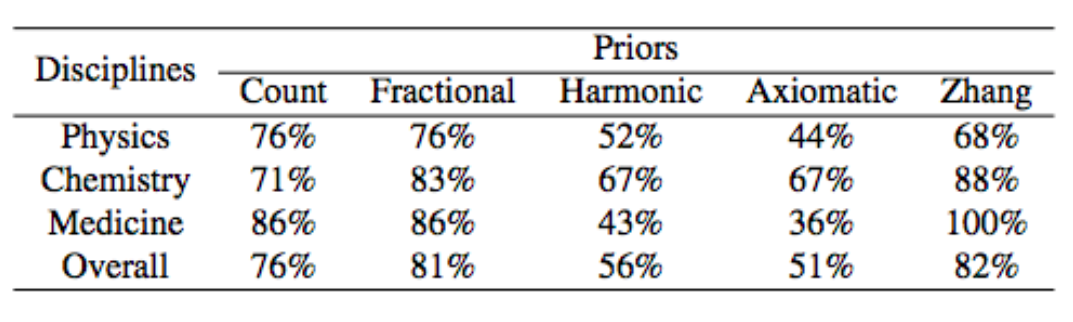
\includegraphics[scale=0.3]{figures/comparison}
\end{figure}
\end{frame}

\begin{frame}{Priors}
\begin{itemize}
\item Count prior: Each author of paper $p_j$ gets one credit.
\[A_{ij} = I\{a_i\in p_j\}\]
\item Fractional Prior: All authors of paper $p_j$ equally share one credit
\[A_{ij}=I\{a_i\in p_j\}/n_j\]
where $n_j$ is the number of coauthors in $p_j$
\item Harmonic Prior: All authors of paper $p_j$ share one credit, where the share of the $i$th author is proportional to the reciprocal of its rank in the author list.
\[
A_{ij}=\frac{1}{i}/\sum_{k=1}^{n_j} \frac{1}{k}.
\]
\end{itemize}
\end{frame}

\begin{frame}{Priors}
\begin{itemize}
\item Axiomatic Prior: All authors of paper $p_j$ share one credit without exogenous information
\[
A_{ij}=\frac{\sum_{k=1}^{n_j} \frac{1}{k}}{n_j}.
\]
\item Zhang's Prior: The total credit of all authors is $3$. The \textbf{first} author and \textbf{corresponding} author each get one credit. The \textbf{remaining} authors placed at rank $i (1\le i\le n_j-2)$ gets credit
\[
A_{ij} = \frac{2(n_j-i)}{(n_j+1)(n_j-2)}
\]
\end{itemize}
\end{frame}

\begin{frame}{Modified}
Total credits $C$ for all papers, including both the cocited and citing papers.

The qualities of the citing papers are also important, because their importance can affect the cocitation strength vector $s$. Let $w_1,w_2,\ldots,w_\ell$ be the importance score of the citing papers. We modify Shen's method with the information:
\[
s'_i = \sum_{j=1}^{\ell} w_i I\{d_i~\textrm{cocites}~p_0,p_j\}.
\]

The importance of a paper is proportional to its total credits earned from all its authors:
\[
\left\{
\begin{array}{rl}
C & = \sum_i w_i,\\ 
w_i & = \sum_j c_{ij}.
\end{array}
\right.
\]

\end{frame}

\begin{frame}{Datasets}
\begin{itemize}
\item
American Physical Society (APS)\\
\small{
- Period: $1893 - 2009$\\
- Papers and citations from all the $11$ journals of APS\\
- $463,348$ papers, $4,710,547$ citations, and $248,738$ authors
}
\item
Web of Science (WOS)\\
\small{
- Period: $1955-2012$\\
- Multidisciplinary\\
- $37,553,657$ papers, $672,321,250$ citations, and $8,724,394$ authors
}
\end{itemize}
\end{frame}

\begin{frame}{Evaluation}
To evaluate the performance, the Nobel-prize winning papers in Physics (1995 - 2013), Chemistry (1998 - 2013), Medicine (2006 - 2013) and Economics (1998 - 2013) are collected to build the citation network. The credit allocation algorithm produces a credit share for each coauthor appeared in the awarding Nobel Prize papers.
\vskip 1em
The experimental results indicated that Sen's method performs very well, and successfully assigns the Nobel-prize winners the highest credit share in the awarding papers.
\end{frame}

\begin{frame}{Further Studies}
\begin{itemize}
\item Integrating both the order of coauthors and the contextual info to design better credit allocation matrix $A=(A_{ij})_{i=m}^{n+1}$
\item Differentiate the values of the citing papers $\mathcal D$ because of the reputation differences, produce more reliable relevance estimation of $s$ (link-analysis based analyze over all papers) 
\item Authors' institutions and contextual text of the citation(definition, ideas)
\end{itemize}
\end{frame}

\begin{frame}[allowframebreaks]
\tiny\bibliography{references}
\bibliographystyle{unsrt}
\end{frame}

\end{document}